\documentclass[10pt]{article}
\usepackage{icmlko}

\icmlmeta{IP 파운데이션 월드모델}{161}{부채를 갚으니 두 잣대가 화해했다}{노트 160이 남긴 부채 --- 다섯 노트가 뒤집힌 열을 보고 있었다. 방향을 반영해 다시 재니 서로 어긋나던 두 잣대가 같은 말을 한다}

\begin{document}

\twocolumn[
\icmlheader

\begin{abstract}
노트 160이 \texttt{entry\_friction} 이 여섯 도메인에서 라벨에 맞춰 뒤집혀
있음을 찾고 부채를 남겼다 --- 노트 155부터 159까지 다섯 노트가 뒤집힌 열에
안 뒤집힌 사전 부호를 대고 있었다. 갚았다. \texttt{lab/lever.py} 에
\texttt{prior\_of(축, 도메인)} 을 넣어 \texttt{axis\_orient.json} 을 읽고
뒤집힌 곳에서는 사전 부호도 뒤집는다. 다시 재니 \textbf{입장 마찰이
돌아왔다} --- 능형에서 0/8이 \textbf{5/8}로, 배깅에서 2/8이 \textbf{6/8}로
올랐다. ``어느 통제로도 안 고쳐지는 축''은 축이 아니라 장부의 문제였다.
전체 표도 움직인다. \textbf{선형 둘이 제일 크게 오른다} --- F6 능형과 F9
순위우도가 78\%에서 \textbf{89\%}로, F10 도메인수축이 64\%에서 75\%로.
배깅은 81\%$\to$86\%, 부스팅은 83\% 그대로다. 크기 가중으로 보면 다섯이
전부 \textbf{91$\sim$93\%}로 모인다. 그리고 제일 중요한 것 ---
\textbf{서로 어긋나던 두 잣대가 화해했다.} 노트 156은 판 $\rho$ 가
``자료 부호''와는 $-$0.872로, ``사전 부호''와는 $+$0.564로 \emph{반대
방향}으로 붙는다고 적었고 그 모순을 설명 못 했다. 방향을 바로잡으니 사전
부호 쪽이 \textbf{$+$0.564에서 $-$0.564로} 뒤집혀 두 잣대가 같은 부호가
된다. \textbf{노트 156의 핵심 --- ``판을 잘 맞힐수록 손잡이를 못 돌린다''
--- 은 이제 두 잣대 모두에서 확인된다.} 판 4 · 5위인 선형 둘이 손잡이
1위이고 판 1 · 2위인 부스팅 둘이 아래다. 모순이었던 것은 현상이 아니라
뒤집힌 열이었다.
\end{abstract}
]

\begin{figure*}[t]
\centering
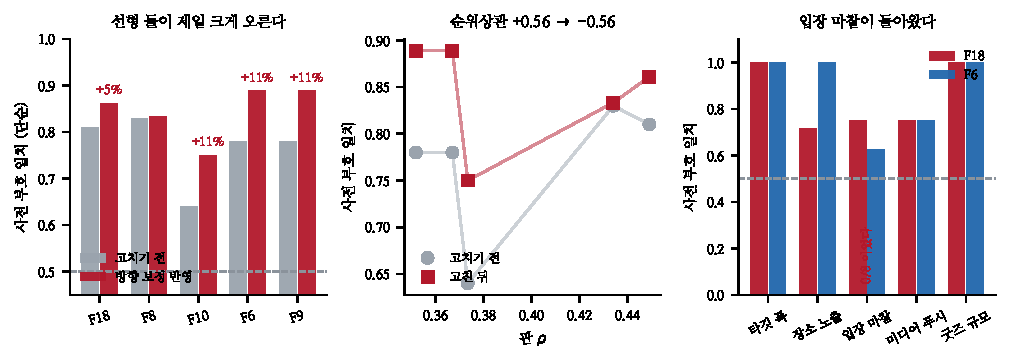
\includegraphics[width=\textwidth]{figs/debt.pdf}
\caption{왼쪽 --- 선형 둘이 제일 크게 오른다. 가운데 --- 판과 부호의 관계가
$+$0.56에서 $-$0.56으로 뒤집힌다. 오른쪽 --- 입장 마찰이 돌아왔다.}
\end{figure*}

\section{장부를 고쳤다}

\texttt{lab/lever.py} 의 사전 부호를 상수에서 함수로 바꿨다.

\begin{table}[t]
\centering\tsize
\caption{사전 부호는 \emph{원 방향} 기준이다.}
\begin{tabular}{ll}
\toprule
이전 & \texttt{PRIOR[axis]} \\
\textbf{이후} & \texttt{PRIOR[axis] $\times$ ($-$1 if 뒤집힌 도메인)} \\
\bottomrule
\end{tabular}
\end{table}

\claimx{\textbf{입장 마찰이 돌아왔다.} 능형 0/8 $\to$ 5/8, 배깅 2/8 $\to$
6/8. 노트 155가 ``내 상식이 틀렸나''를 의심하고 156 · 157 · 158 · 159가
``어느 통제로도 안 고쳐진다''를 반복한 그 축이다.}{여전히 다섯 축 중
제일 낮다(5/8 · 6/8). 방향을 고쳐도 완전히 맞지는 않는다 --- 노트 155의
선택 설명(``유료를 거는 팝업은 원래 수요가 있다'')이 남는다.}

\begin{table}[t]
\centering\tsize
\caption{축별 사전 부호 일치. 방향 보정 반영.}
\begin{tabular}{lrr}
\toprule
& F18 배깅 & F6 능형 \\
\midrule
타깃 폭 & 9/9 & 9/9 \\
굿즈 규모 & 8/8 & 8/8 \\
장소 노출 & 5/7 & \textbf{7/7} \\
\textbf{입장 마찰} & \textbf{6/8} & \textbf{5/8} \\
미디어 푸시 & 3/4 & 3/4 \\
\bottomrule
\end{tabular}
\end{table}

미디어 푸시가 4/4에서 3/4로 내려간 것도 같은 이유다 --- 애니에서
\texttt{media\_push} 도 뒤집혀 있어서(\texttt{axis\_orient.json} 의 두 번째
항목) 사전 부호가 같이 뒤집혔고, 거기서 어긋난다.

\section{표가 움직인다}

\begin{table}[t]
\centering\tsize
\caption{사전 부호 일치. 판 $\rho$ 내림차순.}
\begin{tabular}{lrrrr}
\toprule
& 판 $\rho$ & 전 & \textbf{후} & 가중 \\
\midrule
F18 배깅 & $+$.4491 & 81\% & 86\% & 93\% \\
F8 부스팅 & $+$.4341 & 83\% & 83\% & 92\% \\
F10 도메인수축 & $+$.3735 & 64\% & 75\% & 91\% \\
\textbf{F6 능형} & $+$.3671 & 78\% & \textbf{89\%} & \textbf{93\%} \\
\textbf{F9 순위우도} & $+$.3519 & 78\% & \textbf{89\%} & \textbf{93\%} \\
\bottomrule
\end{tabular}
\end{table}

\claimx{\textbf{선형 둘이 제일 크게 오른다}($+$11\%p). 뒤집힌 열에 제일
크게 벌받던 것이 선형이었다 --- 트리는 부호가 뒤집혀도 분기로 흡수할 수
있지만 선형은 계수 하나가 통째로 뒤집힌다.}{크기 가중으로 보면 다섯이
91$\sim$93\%로 모인다. \textbf{정식화 사이 차이는 크기 가중에서 거의
사라진다} --- 갈리는 것은 작은 칸들이다.}

\section{두 잣대가 화해했다}

노트 156이 모순을 남겼다. 판 $\rho$ 가 ``그 도메인 자료의 부호''와는
$-$0.872로 붙고 ``내 사전 부호''와는 $+$0.564로 붙는다 --- 반대 방향이다.
그때는 ``부스팅이 상식은 따르고 자료는 안 따른다''로 읽었다.

\begin{table}[t]
\centering\tsize
\caption{판 $\rho$ 와의 순위상관.}
\begin{tabular}{lrr}
\toprule
& 고치기 전 & \textbf{고친 뒤} \\
\midrule
사전 부호 일치 & $+$.564 & \textbf{$-$.564} \\
가중 부호 일치 & --- & \textbf{$-$.600} \\
자료 부호 일치 (노트 156) & $-$.872 & --- \\
\bottomrule
\end{tabular}
\end{table}

\claimx{\textbf{모순이 사라진다.} 사전 부호 쪽이 $+$0.564에서 $-$0.564로
뒤집혀 자료 부호 쪽($-$0.872)과 같은 방향이 된다. \textbf{어긋난 것은
현상이 아니라 뒤집힌 열이었다.}}{노트 156이 ``부스팅은 상식을 따르고 자료를
안 따른다''로 붙인 해석은 폐기한다. 실제로는 둘 다 안 따르고, 상식을 따르는
것처럼 보인 이유가 장부 오류였다.}

\claimx{\textbf{그래서 노트 156의 핵심은 더 단단해진다} --- ``판을 잘
맞힐수록 손잡이를 못 돌린다''가 이제 두 잣대 모두에서 확인된다. 판 4 ·
5위인 선형 둘이 손잡이 1위(89\%)이고 판 1 · 2위인 부스팅 둘이 86\% ·
83\%다.}{정식화가 다섯뿐이라 $-$0.564의 표준오차가 크다. 다만 부호가
뒤집힌 것이 아니라 \emph{모순이 해소된} 것이라 방향은 믿을 만하다.}

\begin{table}[t]
\centering\tsize
\caption{남은 것.}
\begin{tabular}{ll}
\toprule
입장 마찰 & 5/8 --- 방향을 고쳐도 제일 낮다 \\
애니 & media\_push 도 뒤집혀 있다 --- 왜 \\
가중 & 다섯이 91$\sim$93\%로 모인다 --- 변별력이 없다 \\
\bottomrule
\end{tabular}
\end{table}

마지막 줄이 다음 잣대 문제다. 크기 가중 부호 일치가 다섯 정식화를 91\%와
93\% 사이에 몰아넣는다. 변별이 안 되면 순위표 열로 못 쓴다 ---
\textbf{단순과 가중 사이 어딘가에 쓸 만한 눈금이 있다.}

\end{document}
